\documentclass[conference]{IEEEtran}
\IEEEoverridecommandlockouts
% The preceding line is only needed to identify funding in the first footnote. If that is unneeded, please comment it out.
\usepackage{cite}
\usepackage{amsmath,amssymb,amsfonts}
\usepackage{algorithmic}
\usepackage{graphicx}
\usepackage{textcomp}
\usepackage{listings}
\usepackage{xcolor}
\usepackage{caption}

\definecolor{codegreen}{rgb}{0,0.6,0}
\definecolor{codegray}{rgb}{0.5,0.5,0.5}
\definecolor{codepurple}{rgb}{0.58,0,0.82}
\definecolor{backcolour}{rgb}{0.95,0.95,0.92}

\lstdefinestyle{mystyle}{
    backgroundcolor=\color{backcolour},   
    commentstyle=\color{codegreen},
    keywordstyle=\color{magenta},
    numberstyle=\tiny\color{codegray},
    stringstyle=\color{codepurple},
    basicstyle=\ttfamily\footnotesize,
    breakatwhitespace=false,         
    breaklines=true,                 
    captionpos=b,                    
    keepspaces=true,                 
    numbers=left,                    
    numbersep=5pt,                  
    showspaces=false,                
    showstringspaces=false,
    showtabs=false,       
    tabsize=1
}
\lstset{style=mystyle}

\def\BibTeX{{\rm B\kern-.05em{\sc i\kern-.025em b}\kern-.08em
    T\kern-.1667em\lower.7ex\hbox{E}\kern-.125emX}}
 \setlength{\parskip}{0.25cm}
\begin{document}

\title{Federated Learning in Outdoor Human Mobility Scenarios\\
}

\author{\IEEEauthorblockN{Dorian-Alexandru Verna}
\IEEEauthorblockA{\textit{Computer Science Department} \\
\textit{University Politehnica of Bucharest}\\
Bucharest, Romania \\
dorianverna7@gmail.com}
}

\maketitle

\begin{abstract}
The exponential growth of IT capabilities involves the development of new software tools, many of which use sensitive or confidential information. Thus, managing Personally Identifiable Information (PII) has become a critical aspect of modern software development. Products must comply with regulations such as GDPR, which set specific rules for the collection, processing, and distribution of such data.

On the other hand, a rapidly expanding branch of the IT field is federated learning. This approach involves training individual machine learning (ML) models on various devices distributed across a specific area (normally belonging to individuals who have provided consent), transmitting the resulting models to a central server, and aggregating them into a more robust model. This enhanced model is then sent back to the devices. Federated learning has many applications today, but in this study we focus on the issue of federated learning in the context of human outdoor mobility. This concept of outdoor mobility refers to the flow of people's movements across relatively large spaces, such as cities. Numerous applications of this idea can be implemented once a viable solution is found.

This study aims to examine, compare, and, where possible, propose alternatives for managing data privacy in the context of federated learning. We will explore methods such as differential privacy approaches, secure aggregation, and homomorphic encryption. In addition, we will analyze the types of data typically transmitted in federated learning and the risks associated with them. Previous studies highlight other methods, such as Secure Function Evaluation (SFE) and Secure Multi-Party Computation (SMC), which will also be analyzed here.

Naturally, the study also includes an analysis of architectural risks, where we will present the existing topologies in federated learning and provide a brief comparison of preferred communication protocols. The topologies may involve connections between the central server and individual devices, as well as the existence of intermediate servers that communicate with devices and then with the central server. The use of proxies will also be addressed, along with other relevant concepts to define the characteristics of a high-quality solution.
\end{abstract}

\section{Introduction}
Human mobility plays a fundamental role in daily activities, involving movement within urban and interurban spaces to achieve various goals. Modern society, compared to the past, emphasizes efficiency and safety in mobility, facilitated by advancements such as mobile phones, wearable devices, and autonomous vehicles. These technologies simplify the monitoring and aggregation of mobility data, enabling the analysis of movement patterns and supporting applications for smart cities.

Smart city solutions leverage mobility data collected through distributed devices for diverse purposes: epidemic control, environmental protection, traffic management, and strategic placement of emergency resources. However, the aggregation of such data raises privacy concerns, as European GDPR regulations prohibit storing or using personal location data without user consent.

To address these challenges, federated learning has emerged as a privacy-compliant solution. This approach involves training predictive models directly on user devices (e.g., mobile phones) while sharing only the aggregated model updates with a central system. This ensures that sensitive data remains local while still enabling accurate mobility predictions.

Federated learning offers effective solutions for challenges in human mobility. During events like the COVID-19 pandemic, it helps predict population movements, allowing authorities to isolate high-risk zones and manage the spread of the virus. It also supports urban planning by forecasting migration trends, aiding in the equitable distribution of resources and opportunities. For traffic management, mobility predictions can optimize public transit and reduce congestion by rerouting flows. Additionally, it improves emergency response by identifying areas likely to need police, ambulance, or firefighting resources. While promising, refining federated learning techniques to enhance efficiency and scalability remains an ongoing research priority.

In the following chapters, we aim to tackle key concepts related to federated learning and how it can be applied to stimulate decisions in terms of outdoor human mobility. In addition, we will tackle the privacy and PII handling known and existent approaches (differential privacy, various encryption algorithms, SFE and SMC), as well as topologies of federated networks that favor the aspect data privacy (centralized or decentralized topologies). A separate chapter involves analyzing existing datasets that would serve as training data for the models proposed afterwards, identifying sensitive information out of the fields present in the data entries. We perform a short comparison of the solutions mentioned previously and draft conclusions on a recommendation of federated learning architecture that would take into account sensitive data handling.

\section{State of the Art}

This chapter delves into these cutting-edge solutions, analyzing their applications, strengths, and limitations within the context of human outdoor mobility. Furthermore, it examines the architectural frameworks and communication protocols that underpin federated learning systems, emphasizing their implications for scalability, efficiency, and privacy preservation.

\subsection{Outdoor Mobility}

There are several prediction algorithms and methods used for analyzing and providing estimations on future locations of a population of individuals, these are referenced by Wang \textit{et al.} [1] and plotted in Figure 1.

\begin{figure}[htbp]
\centerline{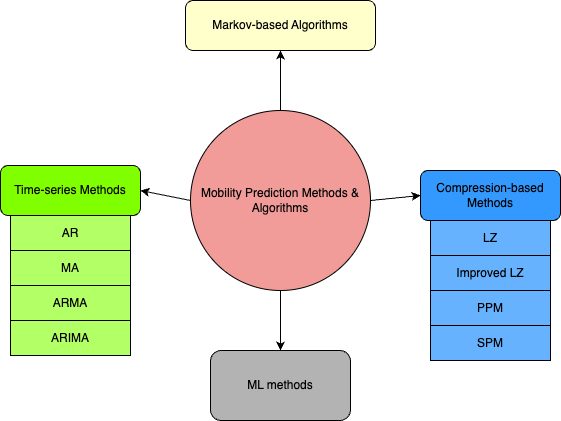
\includegraphics[scale=0.4]{Outdoor_algorithms.png}}
\caption{Outdoor Mobility Prediction Algorithms}
\label{fig}
\end{figure}

As described, there are multiple directions towards which reasearch can focus when it comes to outdoor human mobility:

\subsubsection{Markov-based methods}
Markov-based methods are stochastic models that determine the probabilities of transition from one state to another. They assume that each observation is a state. If the transition depends on the current state, it is a 1st Markov model. If it depends on the current and previous state, it is a 2nd Markov model.

\subsubsection{Compression-based methods}
Compression-based methods include Lempel-Ziv (LZ), improved LZ, Partial Matching (PPM), and Sample Pattern Matching (SPM). They were originally used in compression, these models being similar to the k-th order Markov model, except k can be infinite.

\subsubsection{Time-series methods}
Time-series methods predict future values in a time series of data. They use different techniques to make time series data stationary, improving prediction accuracy. These methods include Autoregressive (AR), Moving Average (MA), Autoregressive Moving Average (ARMA), and Autoregressive Integrated Moving Average (ARIMA).

\subsubsection{Machine learning methods}
Machine learning methods are widely used for human mobility prediction. They utilize statistical techniques to find patterns in data. They can predict the volume of migration flow, the next location, and the corresponding time in the future. Machine learning methods include supervised, semi-supervised and unsupervised learning, and mainly make the classification or regression of inputs.
\subsection{Federated Learning}

From the point of view of existing Federated Learning solutions, we can identify different types of federated networks and compare them using different perspectives. Three of these main categories based on which we can identify current state-of-the-art solutions are based on efficiency in communication, learning methods used, and correctness in terms of data privacy and security.

\subsubsection{Communication Efficiency}

Just as Li \textit{et al.} [2] describes the current state of Federated Learning solutions, the main topologies used are centralized and decentralized topologies. Centralized topologies are also known as Star Networks and usually there is a main server that coordinates the learning process and communicates with all devices. On the other side, the decentralized topology involves a graph-like structure, where each device is able to communicate with neighbors. In terms of efficiency, the decentralized topology would be most useful in low bandwidth and high latency networks, used predominantly when connections are unreliable and set up in an ad-hoc manner.

\begin{figure}[htbp]
\centerline{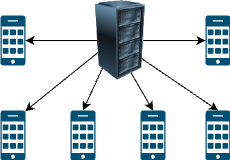
\includegraphics[scale=0.7]{centralized_training.png}}
\caption{Overview of centralized topology}
\label{fig}
\end{figure}

When it comes to security and privacy, the first topology is preferred, as it relies on secure connections to the central server and on the integrity of this central node. Figure 2. and Figure 3 display the these two types of topologies that have been previously described.

\begin{figure}[htbp]
\centerline{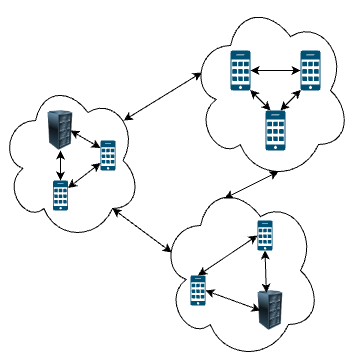
\includegraphics[scale=0.5]{decentralized_training.png}}
\caption{Overview of decentralized topology}
\label{fig}
\end{figure}

\subsubsection{Learning Methods}

There are various algorithms used for model aggregation in federated learning and that guarantee good results. Current State-of-the-Art solutions are based on algorithms like Federated Averaging (FedAvg) [3], which is a foundational optimization algorithm and allows clients to perform multiple local SGD updates on their own data before communicating model updates to the server, FedProx, which is a generalization of FedAvg that takes into account non-IID data, being designed for heterogenous devices, Meta-Learning algorithms that leverage the concept of multi-task learning in order to learn separate models for each device, such as MOCHA [4].

\subsubsection{Data Privacy and Security}

On the privacy and security side, there are a couple of presently used methods that offer good results: differential privacy, Secure Multiparty Computation (SMC), and Homomorphic Encryption.\\\\
\textbf{Differential Privacy} [5] is currently the most popular method for ensuring privacy in federated learning, due to the fact that it offers provable and quantifiable privacy protections, ensuring that the output of an analysis is not significantly affected by the presence or absence of any individual's data. The core idea is based on simplicity adding noise to the data or model updates in order to guard sensitive information that can be extracted. This method also provides lower overhead as compared with the following two methods.\\\\
\textbf{Secure Multiparty Computation} is a cryptographic technique that allows multiple parties to jointly compute a function on their private inputs without revealing those inputs to each other. In the context of Federated Learning, SMC can be used to aggregate model updates from different devices in a secure way. The server would only see the final aggregated result, not the individual updates from each device. Though it guarantees privacy without sacrificing the accuracy of the model, the main limitation resides in the communication overhead, exchange of information can be costly in bandwidth-constrained environments.\\\\
\textbf{Homomorphic Encryption} allows computation to be performed directly on encrypted data without needing to decrypt it first. If applied in Federated Learning, devices could send their encrypted model updates to the server, which can aggregate these encrypted updates and send back the result, still in an encrypted form. While promising, Homomorphic Encryption is not yet widely used in Federated Learning due to some challenges: computational cost, limited aplicability and scalability issues.

\begin{table}[htbp]
\caption{Comparison of various privacy approaches}
\begin{center}
\begin{tabular}{|c|c|c|c|}
\hline
{}& {}& {}& {}\\[-0.5em]
\textbf{Feature}&\textbf{Differential}&\textbf{SMC}&\textbf{Homomorphic} \\
\textbf{}&\textbf{Privacy}&\textbf{}&\textbf{Encryption} \\
{}& {}& {}& {}\\[-0.5em]
\hline
{}& {}& {}& {}\\[-0.5em]
Privacy& Provable& Strong& Potentially \\
{}& {}& {}& Perfect \\
{}& {}& {}& {}\\[-0.5em]
\hline
{}& {}& {}& {}\\[-0.5em]
Accuracy& Minor& No impact& No impact \\
{}& {}& {}& {}\\[-0.5em]
\hline
{}& {}& {}& {}\\[-0.5em]
Overhead& Low& High& Very high \\
{}& {}& {}& {}\\[-0.5em]
\hline
{}& {}& {}& {}\\[-0.5em]
Maturity& Widely used& Actively researched& Early stages \\
{}& {}& {}& {}\\[-0.5em]
\hline
{}& {}& {}& {}\\[-0.5em]
Scalability& Scales well& Challenging& Significant issues \\
{}& {}& {}& {}\\[-0.5em]
\hline
{}& {}& {}& {}\\[-0.5em]
Drawbacks& Slight& High overhead& Cost \& Limited \\
& accuracy loss& & applicability \\
\hline
\end{tabular}
\label{tab1}
\end{center}
\end{table}

A comparison summary of the above discussed privacy approaches can be found in Table 1.

\section{Ethics of Respecting Data Privacy}
Federated Learning deals with sensitive data scattered across many devices, which raises serious concerns. Should any data breach happen, then personal information of an individual and not only (depending on the shared information with the nearby devices) could be exposed. Thus, protecting PII is paramount, but first, we have to be able to identify this type of information. There are multiple identifiers of individuals that federated learning networks have to keep secured:
\begin{itemize}
  \item Direct identifiers:
  \begin{enumerate}
    \item GPS Location Data - core data, but highly sensitive as it can reveal routines, habits, and even personal relationships.
    \item Device IDs - A typical unique identifier that could pose a threat if exposed would be the MAC address or the IMEI identifier.
    \item User Profiles - This category includes lots of personal information that can be linked to mobility, such as age, gender or social connections.\\\\
  \end{enumerate}
  \item Indirect Identifiers:
  \begin{enumerate}
    \item Movement Patterns - Frequent routes, travel times, typical speeds.
    \item Points of Interest - Regular visits to specific locations (gym, restaurant, doctor's office) can reveal sensitive information.
    \item Transportation Modes - Preferred modes (car, bike, public transport) can contribute to identification when combined with other data points.
  \end{enumerate}
\end{itemize}

More specific to the concept of Federated Learning, there could be attackers that aim to manipulate the training process, rather than steal PII. The effect of poisoning the models with bad data can lead to serious consequences on the decisions taken by the authorities in smart cities. For example, attackers can manipulate the distribution or focus of the authorities within a smart city by influencing Federated Learning models to suggest that masses of individuals gather in different zones of the city than the ones that are really of interest.

Finally, the trust users have in Federated Learning solutions is a key fact contributing to the privacy and security enforcement. Most apps that are based on federated learning should specifically ask for the user permissions to make use of the information collected from the individual's device, mentioning what information is collected, guaranteeing the protection of PII data and exposing the risks involved in sharing such information.

\section{Input Data}

A very important aspect in the development of the work is represented by the input data used to train the federated learning network. There are numerous examples of datasets that can be used to predict human mobility outdoors, but not all of these datasets are valid, as they are subject to a series of restrictions under GDPR policies. In this chapter, we will describe the data sources considered in the context of this study.

It is important to note the fact that, though we are presenting two different types of data taken into consideration. The implementation of the solutions are based on the first type of data (randomly generated).

\subsection{Randomly Generated Data}

For the development of a Proof of Concept model (explained later in detail), we chose to use data that reflects the movement of individuals within fictitious points representing well-defined locations in space, intended to cover large areas, such as entire neighborhoods within cities. This organization of data to represent points of interest within urban settlements can serve as a useful abstraction in specific applications that leverage federated learning solutions. For example, in an application that monitors the most frequently visited markets in a city, it is important for the market to be defined as an area of a certain size, and any device located within this area will contribute to generating predictions regarding the likelihood of future visits to that zone by other entities.
Thus, the approach chosen based on the above description makes use of Markov chains and the input data is organized as Markov matrices. An entry in the matrix is the probability for the population to move from one basestation to another basestation. Below there is a snippet of code depicting the way this type of information is generated:

\begin{lstlisting}[language=Python]
def generate_markov_matrix(size):
    matrix = []
    for i in range(size):
        row = [round(random.random(), 3) for _ in range(size)]
        row_sum = sum(row)
        normalized_row = [round(value / row_sum, 3) for value in row]
        matrix.append(normalized_row)
    print(f'Sent matrix: {matrix}')
    return matrix
\end{lstlisting}

An example of Markov transition matrix, based on the code above, is shown in Figure 4., where 0.7 represents the probability of transitioning to state BS1 if the current state is also BS1, 0.3 represents the probability of transitioning to BS2 from BS1, 0.4 defines the transition from BS2 to BS1, and 0.6 specifies the probability of remaining in BS2 if the node was previously in BS2.
\begin{figure}[ht]
\centering
    $\begin{pmatrix}
        0.7 & 0.3 \\
        0.4 & 0.6
    \end{pmatrix}$
\caption{Markov transition matrix}
\end{figure}

\subsection{GNSS Data}
There are numerous scientific studies that focus on examining datasets involving real data related to the position of mobile devices over time. Among these datasets, we can identify collections of data originating from Android devices within Google, known as the High Accuracy GNSS Datasets. The term GNSS refers to the Global Navigation Satellite System, which represents a chipset present in most Android mobile devices that records the position of various devices at specific moments in time. A detailed study of the concepts presented collectively in this paper is described in the study conducted by Fu et al. [6].

This study concentrates on describing this data and on presenting a way to make use of it in further implementations. The code involved in the solutions considered by this study was solely tested on randomly generated data.

An example of how this dataset data is displayed for a particular mobile device, in our case, a Pixel phone, is shown in Figure 5. Basically, to collection of combinations between latitude and longitude points in time for a particular individual device represent a good example of mobility that can be promising in the study of human mobility outdoors.

The most important columns that would serve as input to a ML model considering the issue of outdoor human mobility, while still aligning to the privacy and security requirements of Federated Learning, are represented by coordinates and timestamps. Of course, there is very important to identify whose mobility we are tracking, but this definitely cannot be done by listing the ID of the phone or of the user. A very basic, but good solution would be to hash the identifier of a user, which can be done using various hashing algorithms such as \textbf{MD5} or \textbf{SHA-256}.

\begin{figure}[htbp]
\centerline{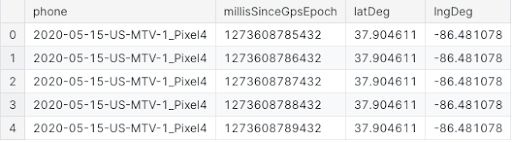
\includegraphics[scale=0.5]{pixel_data.png}}
\caption{Short Display of GNSS Data}
\label{fig}
\end{figure}

One other problem, which concerns privacy and which can lead to easily identify a person is given by the use of coordinates such as latitude and longitude. In the context of using Markov transition matrices, coordinates can be translated to \textbf{basestations}. We refer to a region such as a neighborhood using basestations. This way, a particular person becomes way harder to be identified, due to the fact that the mobility doesn't refer to a specific device anymore, but to a set of devices that are likely to move from one basestation to another.
In order to set up basestations, a cold-start dataset has to be gathered up. Then, using a clusterization method, such as K-means, several points of interest can be identified in a city, these points of interest representing the basestations considered in the context of Markov transition matrices.
A transition matrix changes when there is enough movement identified as to trigger retraining of a model. In that case, the node marks itself as being ready to be chosen by the remote server. Based on percentages of population that moved to a particular basestation, having an origin one, we can determine a probability that can be stored in a transition matrix.

\section{Other Privacy Enhancement Methods}

In this chapter, we explore alternative approaches to enhancing privacy in Federated Learning environments. While traditional methods are well-established, emerging advancements offer innovative ways to further safeguard sensitive information. This chapter focuses on two directions: federated learning server architectures and advanced encryption techniques. Through these approaches, we aim to demonstrate how distributed computation and privacy-preserving algorithms can work synergistically to reduce the risks associated with centralized data storage and processing in the context of training accurate human outdoor mobility predictors.

\subsection{Federated Learning Server Architectures}

One important feature that would surely boost the performance of a federated learning network would be to use a tree topology. A tree-like topology, basically consists of multiple servers that gather, aggregate, sample and communicate aggregated models to client devices that are subject to mobility. All these first-level servers communicate to upper-level servers. This way, the aggregated models are aggregated once again by upper-servers, which most of the times, are guarded by proxy endpoints.

\begin{figure}[htbp]
\centerline{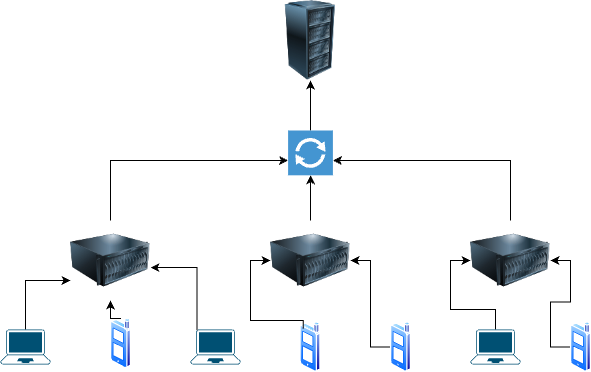
\includegraphics[scale=0.3]{tree_architecture.drawio.png}}
\caption{Overview of tree topology}
\label{fig}
\end{figure}

As to identify both the positive and negative aspects of choosing such a topology, we need to break it down and analyze it gradually:
\begin{itemize}
    \item The usage of multiple servers for aggregation clearly involves various costs to set them up and also set up the communication between such servers, the devices that they sample and share the models' parameters with and the upper level endpoints. On the other hand, having such a distributed infrastructure may lead to better results due to extensive sampling of multiple devices, which can be beneficial to the federated learning network.
    \item Multiple servers can solve the problem of load-balancing and scalability of the system. If a server, becomes overloaded by a very large pool of deviced out of which it should sample, then the load should be redistributed to other servers as well, so that the computational costs don't impact these instances negatively. However, this logic also requires further implementation and, consequently, introduces expenses in terms of synchronization and communication between servers.
    \item Not only are we talking about higher costs in terms of setting up the infrastructure physically, but also when it comes to setting up communication between the server instances and the upper levels of the hierarchy. A change in the code that aggregates the ML models trained would require changing all the servers, which will provoke downtime.
    \item Propagating newly computed ML models from the base levels up to the central server in the top of the hierarchy may involve considerable overhead. This is given by the fact that each server needs to perform aggregation, send the resulting model up the ladder, pass through some proxy instances and take part in constant validation checks. Each of these steps involve a slight overhead which may not be wanted. On the other hand, the propagation goes through various gateways when it comes to this topology, which involves additional security checks.
\end{itemize}

\subsection{Encryption Methods}

There are multiple methods that are treated in this subchapter, most of them are methods considered within the implementation already done or in future implementations of the federated learning network.

\begin{itemize}
    \item Differential Privacy is a very common practice used in Federated Learning. According to Dwork \textit{et al.} [8], differential privacy is a definition rather than a solution or an algorithm. Basically, what DP offers the promise that privacy is ensured by preserving group patterns, without making it possible for adversaries to acquire information about individuals from our datasets. This is achieved by obscuring or adding enough noise to the output of the analysis made using prediction algorithms.
\end{itemize}

Differential Privacy (DP) helps protect client data in federated learning. Two main DP approaches are:
\begin{itemize}
    \item Central Differential Privacy (CDP): The server adds noise to the aggregated model to prevent leaks about individual clients' data. Basically, each client sends an \textit{update} to a central server. To make sure no single client's data has too much influence or reveals sensitive information, these updates are \textit{clipped}. Clipping means setting a maximum limit on how big the update can be. After collecting the clipped updates, the central server mixes some random \textit{noise} to the updates before combining them, thus making sure that it is harder to figure our what any one client contributed.\\
    
    Noise can be added in multiple ways, for example, it can be sampled using the Gaussian distribution with a standard deviation. Several approaches are presented accordingly by McMahan \textit{et al.} [9] and Galen \textit{et al.} [10].\\
    
    \item Local Differential Privacy (LDP): Clients add noise to their data updates before sharing them with the server, ensuring client data remains private.
    Local Differential Privacy ensures that each client performs differential privacy (DP) operations locally, removing the need for a fully trusted aggregator. While LDP enhances privacy compared to central DP, it typically results in reduced accuracy.\\

    Key methods to achieve LDP:
    \begin{itemize}
        \item Adding Noise to Local Updates: Each client adds Gaussian noise to their local updates before sending them to the server, calibrated based on the sensitivity and noise scale.
        \item Adding Noise to Gradients (DP-SGD): During local training, gradients are clipped, and calibrated noise is injected into the gradients to maintain privacy. \\
    \end{itemize}

    We aim to implement LDP in our Flower setup, because the framework has built-in support for Differential Privacy. More details can be found in section \textit{B} of the chapter \textit{VI. Solutions Considered}. \\
\end{itemize}

Hashing PII is a good solution to protect sensitive data, especially in the context of a basic topology such as the ones we are describing in this study. When the complexity scales up, however, we may realize that traditional hashing methods are vulnerable to brute force attacks. Thus, it is worth mentioning that data like phone ID can be hashed using traditional hashing algorithms for now, such as SHA-3, but we should look for better encryption methods in the future. This part is specifically important when we refer to the cold start problem, when we have to perform clustering of the data we have, possibly using K-means.

\section{Solutions considered}

We considered various solutions both when it comes to federated learning and to outdoor mobility prediction. The solutions considered aim to strike a balance between providing good solutions in terms of prediction accuracy and respecting privacy and security requirements.

All solutions considered make use of Markov transition matrices and chain probability as it is a basic model for acquiring knowledge about the future mobility states. What is more, the simplicity of it allows us to concentrate on the privacy concerns of such federated solutions.

\subsection{Proof of Concept}

In the beginning, the aim was to validate that a basic model can be created, along with a very simple topology that would provide predictions about the future positions of individuals in a universe. Thus, the \textit{Proof of concept} solution has been implemented.

The architecture of the project described in this paper consists of a node topology that communicates with a central server, where each node contributes to building a model for predicting outdoor human mobility. This contribution is achieved by training an individual model on each node, transmitting the specific features of the prediction algorithm from each node to the central server, and updating the node's model with the combined features generated at the server level from the previously received models.

The experimental topology initially used consists of only five nodes, one representing the central server and the other four representing individual nodes. In the context of this paper, these nodes simulate the mobile devices of randomly chosen individuals from a population.

Each of the four workers is represented by a Docker container, based on an image built around a Flask application. Similarly, the central node is also represented in the same manner, using a Flask server.

All these instances, created based on Docker images, rely on a configuration made through the docker compose utility. Below, you can see how the topology used in the initial experiment was implemented.

\begin{lstlisting}
  services:
    worker-node-1:
      image: worker-node:latest
      build: ./worker
      ports:
        - "5001:5000"
      depends_on:
        - central-node
      networks:
        - app-network
    worker-node-2:
      image: worker-node:latest
      ports:
        - "5002:5000"
      build: ./worker
      depends_on:
        - central-node
      networks:
        - app-network
<...>
    central-node:
      image: central-node:latest
      build: ./central
      ports:
        - "5005:5000"
      networks:
        - app-network

    networks:
        app-network:
          driver: bridge
\end{lstlisting}

From the perspective of the chosen method for predicting human mobility, we proposed an initial approach based on Markov chains, as the level of complexity in modeling them is lower compared to a Machine Learning model. Higher-complexity prediction algorithms are an important topic addressed in a later section of the paper.

The \textit{Proof of concept} solution makes use of REST APIs for communication between Docker container instances in the discussed work. A worker node sends a transition matrix, containing probabilities of movement between city locations, to the central node via a POST request. In turn, the central node periodically sends POST requests to the worker nodes, enabling each worker to locally aggregate the updated transition matrix provided by the central server. The implementation of the function responsible for sending the transition matrix from the worker to the central node is also outlined below.

\begin{lstlisting}[language=Python]
 def send_data_periodically(interval, size):
    """
    Send data to the central node at regular intervals.


    Args:
        interval (int): The interval in seconds at which data is sent.
        size (int): The size of the sample data list to generate.
    """
    while True:
        matrix = generate_markov_matrix(size)
        response = requests.post(f'{central_node_url}/aggregate', json={'matrices': [matrix]})
        print(f'Sent matrix: {matrix}, Response: {response.json()}')
        time.sleep(interval)
\end{lstlisting}

Though this method serves well in order to provide a basic idea of how a federated learning framework works, there are several aspects that outline the negative aspects of choosing such a solution:
\begin{itemize}
  \item First of all, using a Docker topology generates a lot of memory, CPU and disk space consumption on the nodes that train the models and aggregate them. There is also a additional latency and there can be bottlenecks with regards to the network communication involved in Docker containerization networking.
  \item Secondly, security concerns are considered a very important issue which may be the main negative point of this solution. It is true that Markov chaining provides an abstraction of a population rather than a summary of the movements of a particular individual. Still, Docker containers operate using the Docker daemon and the host kernel. Any vulnerability in the latest two can lead to data leakage. The same problem can arise in the inter-container communication process. Depending on the approach and topology used, network configurations may not be robust enough, such as in the implementation above, leading to further risks.
  \item On the other hand, orchestration, deployment and management of such a topology as the one presented becomes way harder when we want to scale up the number of devices being used. An update to one container may lead to other containers failing and to a considerable amount of downtime. Dependency management issues and version mismatches are problems that we often have to deal with in the context of such software solutions.
\end{itemize}

Validation of results was purely done by analyzing the logs on different Docker containers. The snippet below shows the logs after a Markov transition matrix has been sent from one container and received by the central node. The logs belong to a particular container.

\begin{lstlisting}
Sent matrix: [[0.406, 0.594], [0.501, 0.499]]
Response matrix: {'aggregated_matrix': [[0.388, 0.611], [0.556, 0.443]], 'status': 'aggregated'}
\end{lstlisting}

\subsection{Federated Learning Flower Approach}

There are a couple of software solutions that represent good alternatives to ease the development of Federated Learning. We can also refer to those as frameworks or libraries, the most popular being: Flower, TensorFlow Federated and PySyft. Though all these technologies are worth mentioning, the implementation described in this chapter focuses only on the first one.

As described by Beutel \textit{et al.} [7], Flower represents an open-source FL framework that supports heterogenous environments (mobile and edge devices included). It can also scale to large number of distributed clients while providing flexibility to experiment with novel approaches.

At first, what we have done was to migrate all the \textit{Proof of concept} implementation to a Flower-based approach. The following code snippet depict the steps that the server does in order to send transition matrices to a variable number of clients, and to aggregate the responses from these clients.

\begin{lstlisting}[language=Python]
app = ServerApp()

@app.main()
def main(driver: Driver, context: Context) -> None:
    # Configure the basic server settings
    num_rounds = <...>
    min_nodes = <...>
    fraction_sample = <...>

    for server_round in range(num_rounds):
        # sample the nodes included in round
        while len(all_node_ids) < min_nodes:
            <perform node sampling>
            
        # Create messages
        recordset = RecordSet()
        messages = []

        # Create random markov matrix for coldstart
        params = <...>
        recordset.parameters_records[<...>] = params

        for id in node_ids:
            message = driver.create_message(id, ...)
            messages.append(message)

        # Send messages and wait for all results
        replies = driver.send_and_receive(messages)
        aggregated_matrix = aggregate(replies)
\end{lstlisting}

The key concepts that have been implemented here and cannot be found in the \textit{Proof of concept} solution are:
\begin{itemize}
  \item Sampling of the nodes - Each node in our implementation has an \textit{id} which is sampled using \textit{random} package in Python. This helps when it comes to a large number of nodes. Communication with a very large number of devices is a very costly process for the server, and sampling comes as a good solution. The model we are using is similar to the eventual consistency model, because, at some point in the future, every node will contain the new model.
  \item Performing LDP - Flower has the built-in option of using LDP, which makes it simple to use. Basically, we only had to specify that the \textit{ClientApp} object makes use of a \textit{LocalDpMod} object, which takes as parameters variable like clipping norm value, sensitivity, epsilon, and delta. The code below stands for the change introduced in the code.
  
\begin{lstlisting}[language=Python]
# Add Local Differential Privacy Configuration
local_dp_obj = LocalDpMod(ct.clipping_norm, ct.sensitivity, ct.epsilon, ct.delta)

# Create Client App
app = ClientApp(mods=[local_dp_obj])
\end{lstlisting}

  \item Scaling up and down the number of nodes - This has been done by constantly changing the configurations in the main function of the server-side implementation. Basically the parameter \textit{min\_nodes}, as well as the \textit{fraction\_sample} and \textit{num\_rounds} are very important with respect to this point. Scaling up and down helps in validating whether the solution works for multiple devices, due to the fact that, normally, in the context of outdoor mobility, we have to work with large chunks of data collected from multiple sources.
\end{itemize}

\subsection{Cold-Start Dataset Construction}

{\color{red}TODO - pending, depends on all the other TODOs}

\section{Conclusions}



\begin{thebibliography}{00}
\bibitem{b1} Wang, Jinzhong \& Kong, Xiangjie \& Xia, Feng \& Sun, Lijun. (2019). Urban Human Mobility: Data-Driven Modeling and Prediction. ACM SIGKDD Explorations Newsletter. 21. 1-19. 10.1145/3331651.3331653. 
\bibitem{b2} Li, Tian \& Sahu, Anit \& Talwalkar, Ameet \& Smith, Virginia. (2019). Federated Learning: Challenges, Methods, and Future Directions. 
\bibitem{b3} Juwon Park, Daegun Yoon, Sangho Yeo, Sangyoon Oh. (2022). AMBLE: Adjusting mini-batch and local epoch for federated learning with heterogeneous devices, Journal of Parallel and Distributed Computing, Volume 170, https://doi.org/10.1016/j.jpdc.2022.07.009.
\bibitem{b4} V. Smith, C.-K. Chiang, M. Sanjabi, and A. Talwalkar, “Federated multi-task learning,” in Proc. Advances in Neural Information Processing Systems, 2017, pp. 4424–4434.
\bibitem{b5} C. Dwork and A. Roth. The algorithmic foundations of differential privacy. Foundations and Trends in Theoretical Computer Science, 9:211-407, 2014.
\bibitem{b6} Fu, Guoyu (Michael), Khider, Mohammed, van Diggelen, Frank, "Android Raw GNSS Measurement Datasets for Precise Positioning," Proceedings of the 33rd International Technical Meeting of the Satellite Division of The Institute of Navigation (ION GNSS+ 2020), September 2020, pp. 1925-1937. https://doi.org/10.33012/2020.17628
\bibitem{b7} Beutel DJ, Topal T, Mathur A, Qiu X, Fernandez-Marques J, Gao Y, Sani L, Li KH, Parcollet T, Buarque de Gusmão PP. Flower: A friendly federated learning research framework.
arXiv. 2022. https://doi.org/10.48550/arXiv.2007.14390
\bibitem{b8} Dwork, Cynthia \& Roth, Aaron. (2013). The Algorithmic Foundations of Differential Privacy. Foundations and Trends in Theoretical Computer Science. 9. 10.1561/0400000042. 
\bibitem{b9} McMahan, H. \& Ramage, Daniel \& Talwar, Kunal \& Zhang, Li. (2017). Learning Differentially Private Language Models Without Losing Accuracy. 10.48550/arXiv.1710.06963.
\bibitem{b10} Geyer, Robin \& Klein, Tassilo \& Nabi, Moin. (2017). Differentially Private Federated Learning: A Client Level Perspective. 10.48550/arXiv.1712.07557.

\end{thebibliography}
\vspace{12pt}

\end{document}
